Consider a scalar Toeplitz operator $L_h$ on an infinite one dimensional uniform grid $G_h$,
\begin{equation}
\begin{split}
L_h \mathrel{\hat{=}} \left[ s_\kappa \right]_h \left( \kappa \in V \right)\\
L_h w_h \left( x \right) = \sum_{\kappa \in V} s_\kappa w_h \left( x + \kappa h \right)
\end{split}
\end{equation}
where $V \subset \mathbb{Z}$ is a finite index set, $s_\kappa \in \mathbb{R}$ are constant coefficients, and $w_h \left( x \right)$ is a $l^2$ function on $G_h$.

Since $L_h$ is Toeplitz, it can be diagonalized by the standard Fourier modes $\varphi \left( \theta, x \right) = e^{\imath \theta x / h}$.

\begin{definition}[Symbol of $L_h$]\label{def:symbol}
If for all grid functions $\varphi \left( \theta, x \right)$ we have
\begin{equation}
L_h \varphi \left( \theta, x \right) = \tilde{L}_h \left( \theta \right) \varphi \left( \theta, x \right)
\end{equation}
then we define $\tilde{L}_h \left( \theta \right) = \sum_{\kappa \in V} s_\kappa e^{\imath \theta \kappa}$ as the symbol of $L_h$.
\end{definition}

This definition can be extended to a $p \times p$ linear system of operators by
\begin{equation}
\tilde{\mathbf{L}}_h =
\begin{bmatrix}
    \tilde{L}_h^{1, 1} && \cdots && \tilde{L}_h^{1, p} \\
    \vdots             && \vdots && \vdots             \\
    \tilde{L}_h^{p, 1} && \cdots && \tilde{L}_h^{p, p} \\
\end{bmatrix}
\end{equation}
where $\tilde{L}_h^{i, j}$, $i, j \in \left[1, 2, \dots, p \right]$ is given by scalar Toeplitz operators describing how component $j$ appears in the equation for component $i$.

Note that for a system of equations representing an error propagation operator in a relaxation scheme, the spectral radius of the symbol matrix determines now rapidly the scheme decreases error at a target frequency.
Low frequencies are given by $\theta \in T^{\text{low}} = \left[ - \pi / 2, \pi / 2 \right)$ and high frequencies are given by $\theta \in T^{\text{high}} = \left[ - \pi / 2, 3 \pi / 2 \right) \setminus T^{\text{low}}$.

We can compute the symbol of a $p \times p$ linear system of operators representing a discretized PDE.
We start with a system of equations representing a Galerkin operator, such as in Equation \ref{eq:jacobian_form}.
We omit boundary terms, as they are not present on the infinite uniform grid $G_h$.

Using the algebraic representation of PDE operators given in Chapter \ref{ch:HighOrderFEM}, the PDE operator ${\color{burgundy}\mathbf{A}}$ is of the form
\begin{equation}
\begin{tabular}{c}
${\color{burgundy}\mathbf{A}} = \mathbf{P}^T \mathbf{G}^T {\color{burgundy}\mathbf{A}}^e \mathbf{G} \mathbf{P}$\\
${\color{burgundy}\mathbf{A}}^e = {\color{blue(ncs)}\mathbf{B}}^T {\color{applegreen}\mathbf{D}} {\color{blue(ncs)}\mathbf{B}}$
\end{tabular}
\label{eq:localoperator}
\end{equation}
where $\mathbf{P}$ and $\mathbf{G}$ represent the element assembly operators, ${\color{blue(ncs)}\mathbf{B}}$ is a basis operator which computes the values and derivatives of the basis functions at the quadrature points, and ${\color{applegreen}\mathbf{D}}$ is a block diagonal operator which provides the pointwise application of the bilinear form on the quadrature points, to include quadrature weights and the change in coordinates between the physical and reference space.

We focus on Fourier analysis of the local element operator, ${\color{burgundy}\mathbf{A}}^e$.
The nodes on the left and right boundaries of the element map to the same Fourier mode due to periodicity, so we can compute the symbol matrix as
\begin{equation}
\tilde{{\color{burgundy}\mathbf{A}}} = \mathbf{Q}^T \left( {\color{burgundy}\mathbf{A}}^e \odot \left[ e^{\imath \left( x_i - x_j \right) \theta / h} \right] \right) \mathbf{Q}
\end{equation}
where $\odot$ represents pointwise multiplication of the elements, $h$ is the length of the element, and $i, j \in \left[ 0, 1, \dots, p\right]$.
$\mathbf{Q}$ is a $\left( p + 1 \right) \times p$ matrix that localizes Fourier modes to each element.
\begin{equation}
\mathbf{Q} =
\begin{bmatrix}
    \mathbf{I}   \\
    \mathbf{e}_0 \\
\end{bmatrix} =
\begin{bmatrix}
    1      && 0      && \cdots && 0      \\
    0      && 1      && \cdots && 0      \\
    \vdots && \vdots && \vdots && \vdots \\
    0      && 0      && \cdots && 1      \\
    1      && 0      && \cdots && 0      \\
\end{bmatrix}
\label{eq:fouriermodelocalization1d}
\end{equation}

The computation of this symbol matrix extends to more complex PDE with multiple components and in higher dimensions.

Multiple components are supported by extending the $p \times p$ system of Toeplitz operators in Equation \ref{eq:fouriermodelocalization1d} to a $\left( p \cdot n \right) \times \left( p \cdot n \right)$ system of operators, where $n$ is the number of components.

The infinite uniform grid $G_h$ is extended into higher dimensions by taking the direct sum of the one dimensional grid.
In a similar fashion to how tensor products are used to extend the one dimensional bases into higher dimensions, the localization of Fourier modes in two dimensions is given by
\begin{equation}
\mathbf{Q}_{\text{2d}} = \mathbf{Q} \otimes \mathbf{Q}
\end{equation}
and the localization in three dimensions is given by
\begin{equation}
\mathbf{Q}_{\text{3d}} = \mathbf{Q} \otimes \mathbf{Q} \otimes \mathbf{Q}.
\end{equation}
In general, we will omit the subscript indicating the dimension of the Fourier mode localization operator.

\begin{definition}
The symbol matrix of a finite element operator for an arbitrary second order PDE with any number of components, basis order, and dimension is given by
\begin{equation}
\tilde{{\color{burgundy}\mathbf{A}}} \left( \mathbf{\theta} \right) = \mathbf{Q}^T \left( {\color{burgundy}\mathbf{A}}^e \odot \left[ e^{\imath \sum_d \left( \mathbf{x}_i - \mathbf{x}_j \right) \mathbf{\theta} / \mathbf{h}} \right] \right) \mathbf{Q}
\label{eq:symbolhighorder}
\end{equation}
where $\odot$ represents pointwise multiplication of the elements, $\mathbf{h}$ is the length of the element in each dimension, $\mathbf{\theta}$ is the target frequency in each dimension, $i, j \in \left[ 0, 1, \dots, p^d \right]$, and $d$ is the dimension of the finite element basis.
${\color{burgundy}\mathbf{A}}^e$ is the finite element operator for the element and $\mathbf{Q}$ is the localization operator for Fourier modes on an element.
\label{def:high_order_symbol}
\end{definition}

Note that this LFA notation is applicable to any second-order PDE with a weak form that can be represented by Equation \ref{eq:jacobian_form}.
This representation is used in \href{https://www.github.com/jeremylt/LFAToolkit.jl}{LFAToolkit.jl}, where the users provide the finite element basis ${\color{blue(ncs)}\mathbf{B}}$, the node to mode mapping $\mathbf{Q}$, and the pointwise representation of the weak form ${\color{applegreen}\mathbf{D}}$, and the software can provide the LFA of the PDE with various preconditioners.

As we develop LFA of various preconditioners and smoothers in this notation throughout this chapter, we will the standard test problem of the scalar diffusion operator to illustrate the properties of this analysis for these techniques.

\begin{figure}[!h]
  \centering
  \subfloat[Spectrum of Scalar Diffusion for $p = 4$]{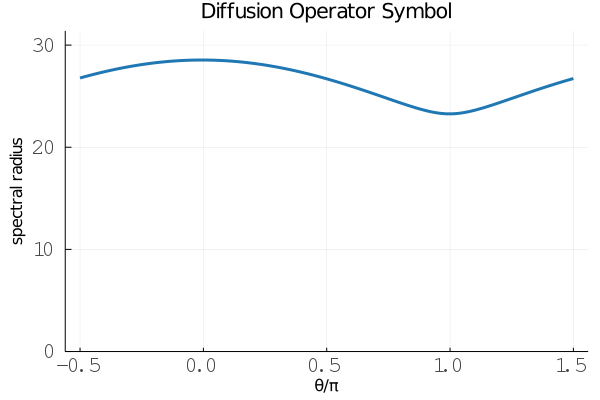
\includegraphics[width=0.48\textwidth]{../img/diffusionSymbol1D}\label{fig:diffusion_spectrum_1d}}
  \hfill
  \subfloat[Spectrum of Scalar Diffusion for $p = 4$]{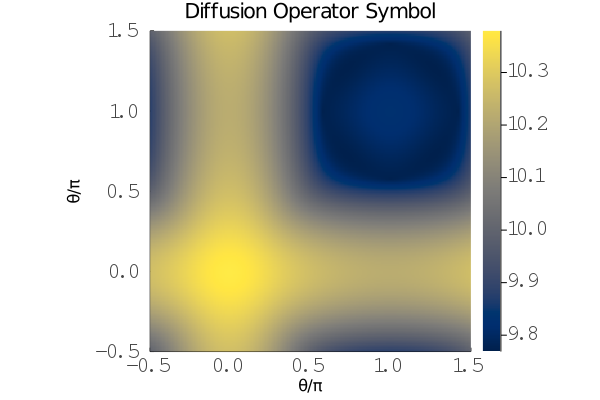
\includegraphics[width=0.48\textwidth]{../img/diffusionSymbol2D}\label{fig:diffusion_spectrum_2d}}
  \caption{Spectrum of Scalar Diffusion Operator Symbol}
\end{figure}

In Figures \ref{fig:diffusion_spectrum_1d} and \ref{fig:diffusion_spectrum_2d}, we see the spectral radius of the symbol of scalar diffusion operator with a fourth-order H1 Lagrange finite element basis on the Gauss-Lobatto points in one and two dimensions.
These plots were generated with \href{https://www.github.com/jeremylt/LFAToolkit.jl}{LFAToolkit.jl}.
Various preconditioning techniques will reduce this spectral radius, with different effectiveness in different frequency ranges.
